\documentclass[authoryear,5p]{elsarticle}

\renewcommand{\today}{}  % Get rid of date on footer
\journal{Ann. Nucl. Energy}

\usepackage[bitstream-charter]{mathdesign} % Use BT Charter font
\usepackage[T1]{fontenc}                   % Use T1 encoding instead of OT1
\usepackage[utf8]{inputenc}                % Use UTF8 input encoding
\usepackage{microtype}                     % Improve typography
\usepackage{amsmath, mathtools}             % AMS Math extensions
\usepackage{booktabs}                      % Improved table spacing
\usepackage{booktabs}
\usepackage{siunitx}
\usepackage{breqn}
\usepackage{nicefrac}

\usepackage[breaklinks=true]{hyperref}

\usepackage{subcaption}
\usepackage{dblfloatfix}
\usepackage{color}

\usepackage{todonotes}

\usepackage[labelfont=bf]{caption}
\captionsetup[figure]{labelsep=period, name=Figure}
\captionsetup[table]{labelsep=period, name=Table}
\def \figureautorefname {Figure}
\def \algorithmautorefname {Algorithm}

\usepackage[scaled]{beramono}

\usepackage{etoolbox}
\usepackage{listings}
\usepackage{color}

% Algorithm constructs
\usepackage{algorithm} % Provides algorithm environment
\usepackage{algorithmicx}       % Provides algorithmic block
\usepackage{algpseudocode}      % Option of algorithmicx package
\renewcommand{\thealgorithm}{\thechapter-\arabic{algorithm}}
\newcommand\Algphase[1]{%
\vspace*{-.7\baselineskip}\Statex\hspace*{\dimexpr-\algorithmicindent-2pt\relax}\rule{\columnwidth}{0.4pt}%
\Statex\hspace*{-\algorithmicindent}{#1}%
\vspace*{-.7\baselineskip}\Statex\hspace*{\dimexpr-\algorithmicindent-2pt\relax}\rule{\columnwidth}{0.4pt}%
}
\newcommand{\algrule}[1][.4pt]{\par\vskip.5\baselineskip\hrule height #1\par\vskip.5\baselineskip}

\newcommand{\code}[2]{
  \subsection*{#1}
  \lstinputlisting{#2}
}

\def\sectionautorefname{Sec.}
\def\subsectionautorefname{Sec.}
\def\subsubsectionautorefname{Sec.}
\def\equationautorefname{Eq.}
\def\figureautorefname{Fig.}
\def\algorithmautorefname{Alg.}

% Patch to make equation autoref counter work
\makeatletter
\patchcmd\eq@setnumber{\stepcounter}{\refstepcounter}{}{%
  \errmessage{Patching \noexpand\eq@setnumber failed}%
}
\makeatother

\hypersetup{colorlinks=true,
  pdftitle={The Impact of Spatial Self-Shielding on Pin-wise Reaction Rates},
  pdfauthor={William Boyd, Benoit Forget and Kord Smith.}}

\begin{document}

\begin{frontmatter}

\title{The Impact of Spatial Self-Shielding on Pin-wise Reaction Rates}

\author{William Boyd\corref{cor1}}
\ead{wboyd@mit.edu}

\author{Benoit Forget\corref{}}
\ead{bforget@mit.edu}

\author{Kord Smith\corref{}}
\ead{kord@mit.edu}

\address{Massachusetts Institute of Technology, Department of Nuclear Science and Engineering, 77 Massachusetts Avenue, Building 24, Cambridge, MA 02139, United States\vspace{-8ex}}


%%%%%%%%%%%%%%%%%%%%%%%%%%%%%%%%%%%%%%%%%%%%%%%%%%%%%%%%%%%%%%%%%%%%%%%%%%%%%%%
\begin{abstract}
%%%%%%%%%%%%%%%%%%%%%%%%%%%%%%%%%%%%%%%%%%%%%%%%%%%%%%%%%%%%%%%%%%%%%%%%%%%%%%%

\end{abstract}

\begin{keyword}
Multi-group cross-sections, spatial homogenization, spatia self-shielding
\end{keyword}

\end{frontmatter}

%%%%%%%%%%%%%%%%%%%%%%%%%%%%%%%%%%%%%%%%%%%%%%%%%%%%%%%%%%%%%%%%%%%%%%%%%%%%%%%
\section{Introduction}
\label{sec:intro}
%%%%%%%%%%%%%%%%%%%%%%%%%%%%%%%%%%%%%%%%%%%%%%%%%%%%%%%%%%%%%%%%%%%%%%%%%%%%%%%

The nuclear reactor physics community has long strived for deterministic neutron transport-based tools for whole-core reactor analysis. A key challenge for whole-core multi-group transport methods is accurate reactor agnostic multi-group cross section (MGXS) generation. The MGXS generation process applies a series of approximations to produce spatially homogenized and energy condensed MGXS in each spatial zone and energy group. ... However, the practical impact of ... is less understood. This paper investigates the ... and quantifies its significance for heterogeneous PWR problems.

This work employs Monte Carlo (MC) neutron transport simulations to generate MGXS. Monte Carlo methods have increasingly been used to generate few group constants for coarse mesh diffusion, most notably by the Serpent MC code \citep{serpent2013manual}, and to a much lesser extent, for high-fidelity neutron transport methods~\citep{redmond1997multigroup, nelson2014improved, cai2014condensation, boyd2016thesis}. The advantage of a MC-based approach is that all of the relevant physics are directly embedded into MGXS by weighting the continuous energy cross sections with a statistical proxy to the ``true'' neutron flux. 

This paper seeks to identify the bias between continuous energy and multi-group transport methods for MGXS libraries which account for spatial self-shielding effects\footnote{The effects of neighboring pins, burnable poisons, reflectors and the core baffle are each of interest in the context of spatial self-shielding.} to varying degrees. In particular, this paper quantifies the difference in the approximation error between simulations in which the same MGXS are used in each unique fuel pin (\textit{e.g.}, each fuel enrichment) and those in which unique MGXS are used in each and every pin. The former case does little if anything to model spatial self-shielding effects, whereas the latter case ``fully'' resolves these effects, albeit at the expense of very large MGXS libraries.

% This difference in approximation error motivates the development of a novel methodology in the following chapters which uses statistical clustering to capture spatial self-shielding effects in MGXS.

The content in this paper is organized as follows. Two different schemes for spatial homogenization of pin-wise MGXS are introduced in~\autoref{sec:methodology}. The need for a new, more flexible and specialized approach to spatial homogenization which appropriately captures spatial self-shielding effects with minimal computational expense is discussed in~\autoref{sec:conclusions}.
%%%%%%%%%%%%%%%%%%%%%%%%%%%%%%%%%%%%%%%%%%%%%%%%%%%%%%%%%%%%%%%%%%%%%%%%%%%%%%%
\section{Methodology}
\label{sec:methodology}
%%%%%%%%%%%%%%%%%%%%%%%%%%%%%%%%%%%%%%%%%%%%%%%%%%%%%%%%%%%%%%%%%%%%%%%%%%%%%%%

%%%%%%%%%%%%%%%%%%%%%%%%%%%%%%%%%%%%%%%%%%%%%%%%%%%%%%%%%%%%%%%%%%%%%%%%%%%%%%%
\subsection{Continuous Energy Calculations with OpenMC}
\label{subsec:openmc}

-OpenMC~\cite{romano2013openmc}
-Python API~\cite{boyd2016bigdata}
-NNDC data~\cite{nndc2016endf}
-distribcell tallies~\cite{lax2014distribcell}
-\texttt{openmc.mgxs}
  -tallied in CASMO's seventy energy group structure~\cite{rhodes2006casmo}
-iso-in-lab
-runtime parameters:
  -num. particles, batches
  -computer hardware

%%%%%%%%%%%%%%%%%%%%%%%%%%%%%%%%%%%%%%%%%%%%%%%%%%%%%%%%%%%%%%%%%%%%%%%%%%%%%%%
\subsection{Multi-Group Calculations with OpenMOC}
\label{subsec:openmoc}

-OpenMOC~\cite{boyd2014openmoc}
-multi-core parallelism~\cite{boyd2016parallel}
-runtime parameters:
  -azim angles, spacing
  -num. FSRs
  -CMFD energy and spatial mesh
  -computer hardware


%%%%%%%%%%%%%%%%%%%%%%%%%%%%%%%%%%%%%%%%%%%%%%%%%%%%%%%%%%%%%%%%%%%%%%%%%%%%%%%
\subsection{Pin-wise Spatial Homogenization Schemes}
\label{subsec:homogenize}

-focus less on introducing these as ``schemes'' per se
  -rather two spatial self-shielding models to quantify approx. error

This paper employs two different spatial homogenization schemes to model spatial self-shielding effects in MGXS. Although all spatial zones may experience spatial self-shielding, this chapter only models the impact of spatial self-shielding on MGXS in fissile regions. The null and degenerate spatial homogenization schemes are introduced in~\autoref{subsubsec:homogenize-null} and~\autoref{subsubsec:homogenize-degenerate}, respectively. These schemes model spatial self-shielding for each fuel pin with increasing granularity and complexity. A fuel assembly and 2$\times$2 colorset with reflector model are color-coded by material and illustrated in Fig.~\ref{fig:homogenization-schemes} for each homogenization scheme.

\begin{figure*}[h!]
\centering
\begin{subfigure}{0.45\textwidth}
  \centering
  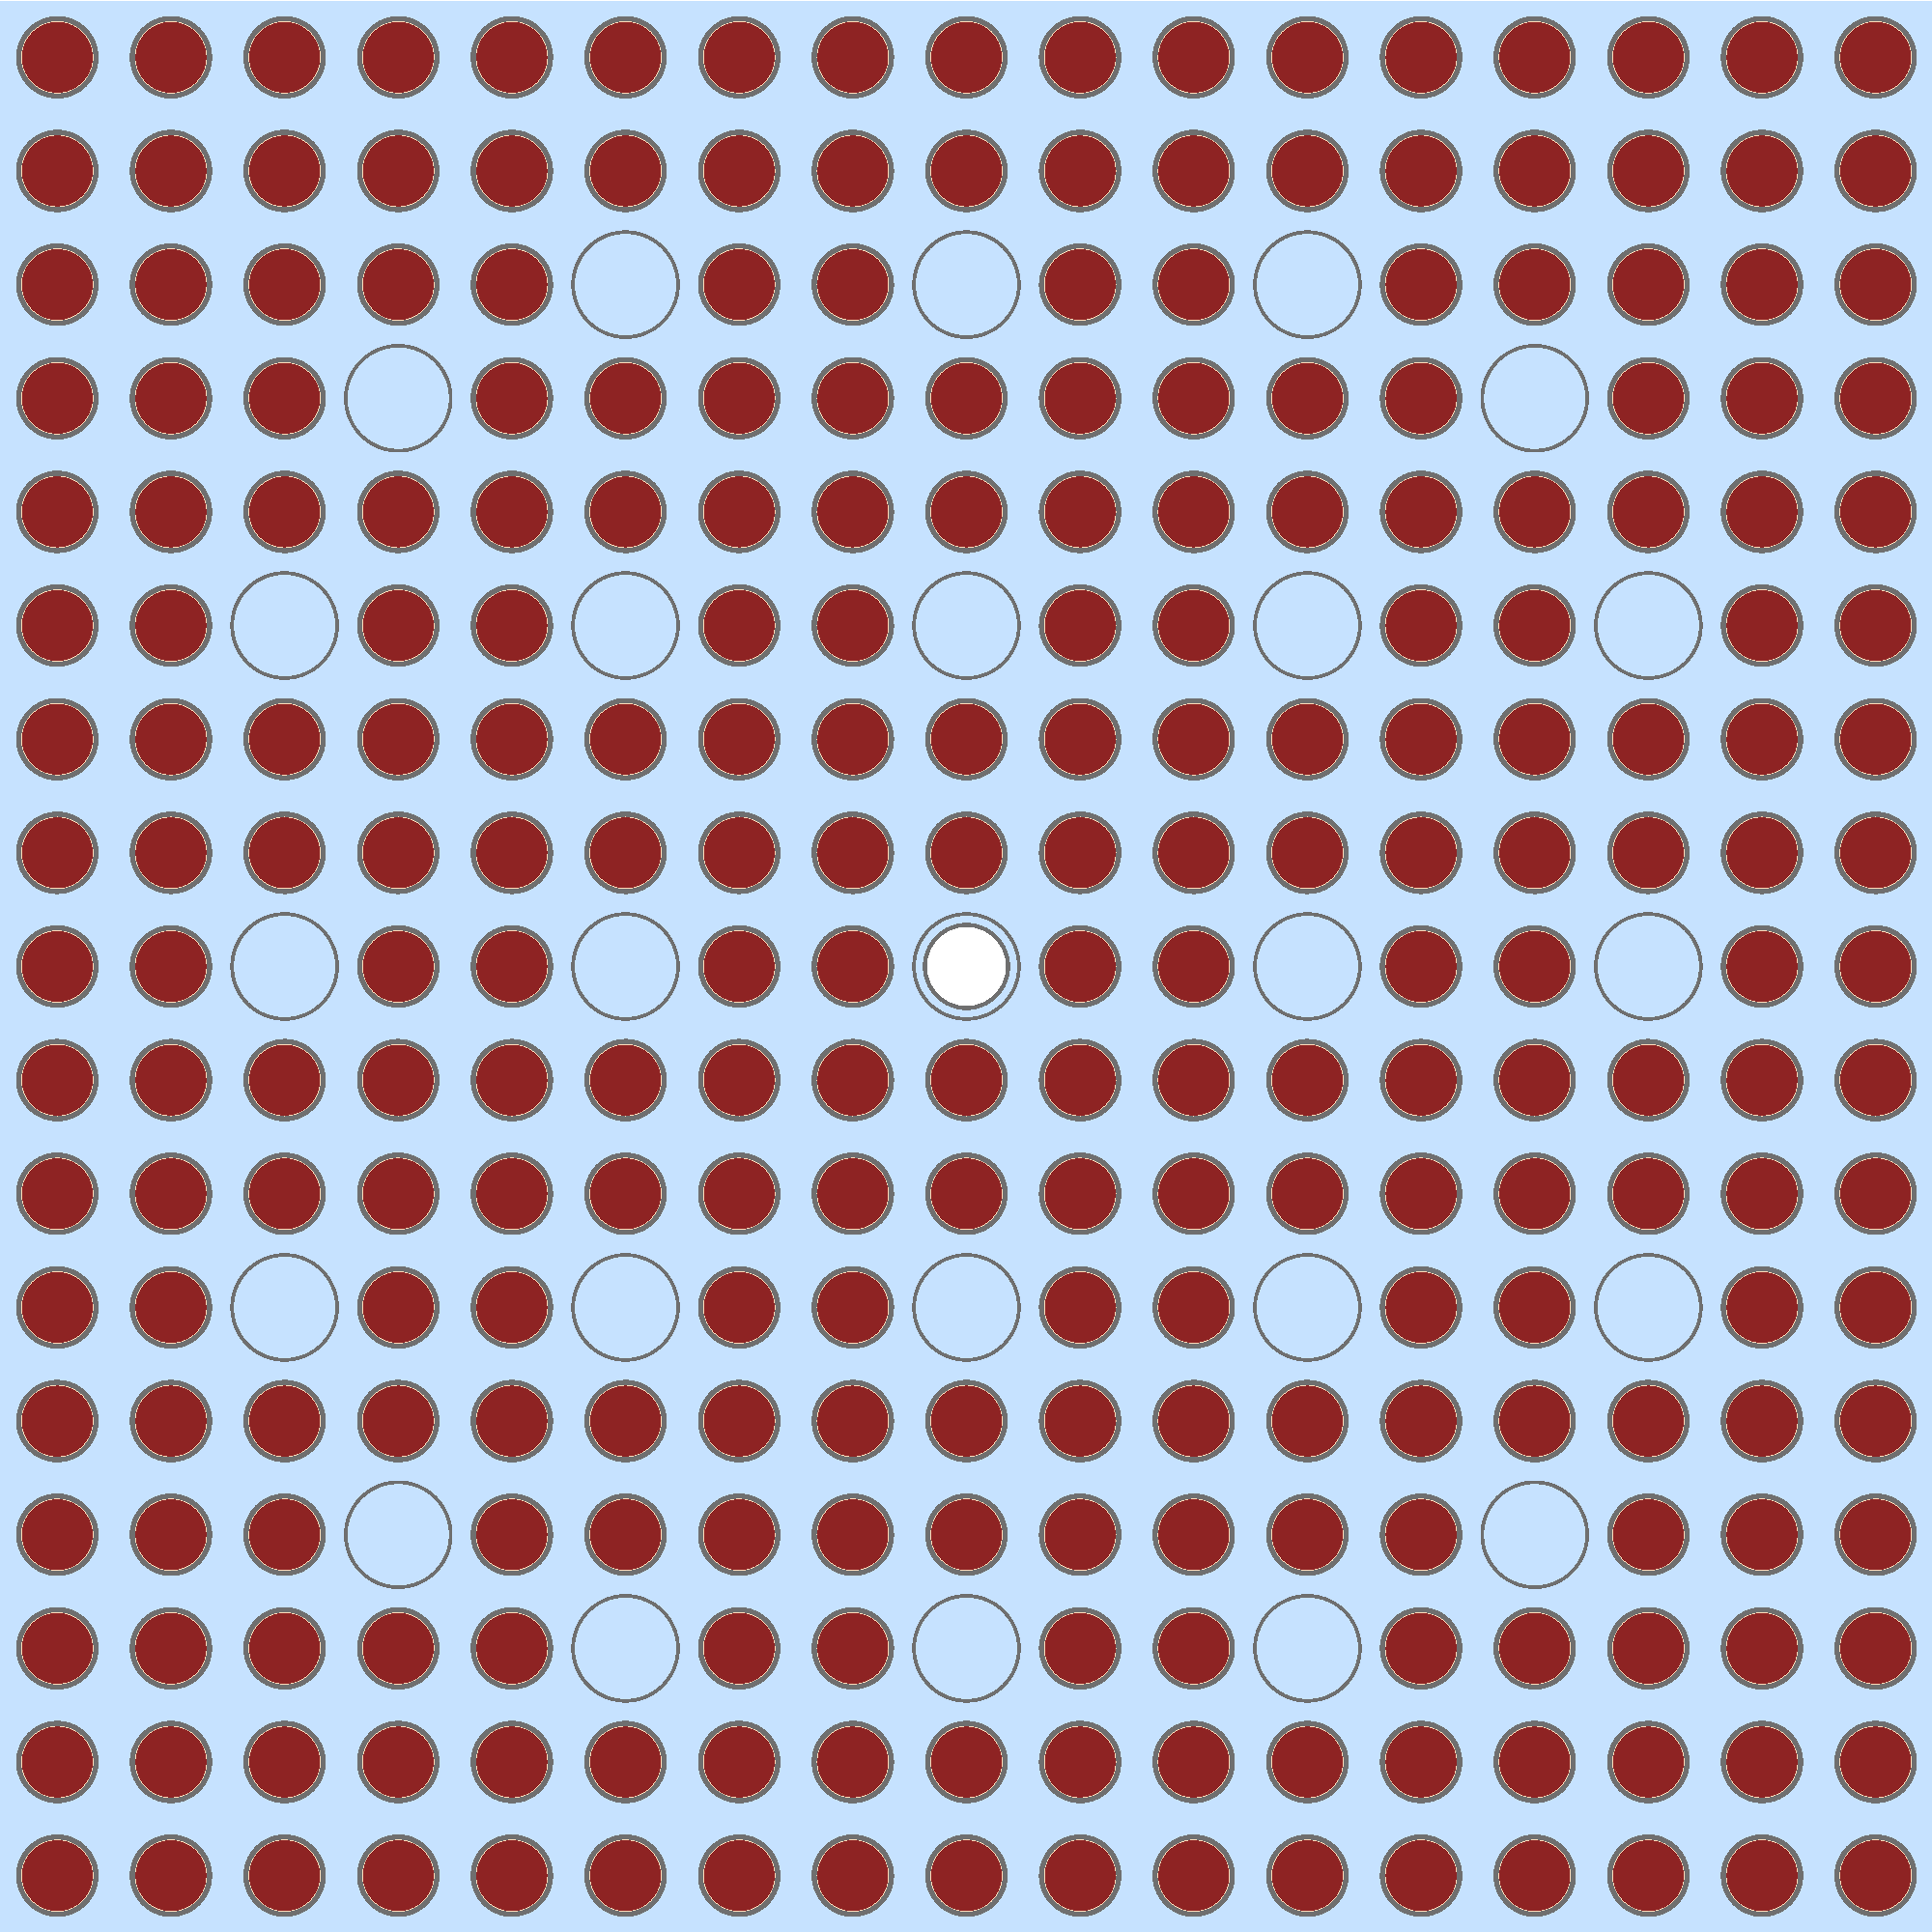
\includegraphics[width=0.8\linewidth]{figures/assembly/geometry}
  \caption{}
  \label{fig:null-assm}
\end{subfigure}
\begin{subfigure}{0.45\textwidth}
  \centering
  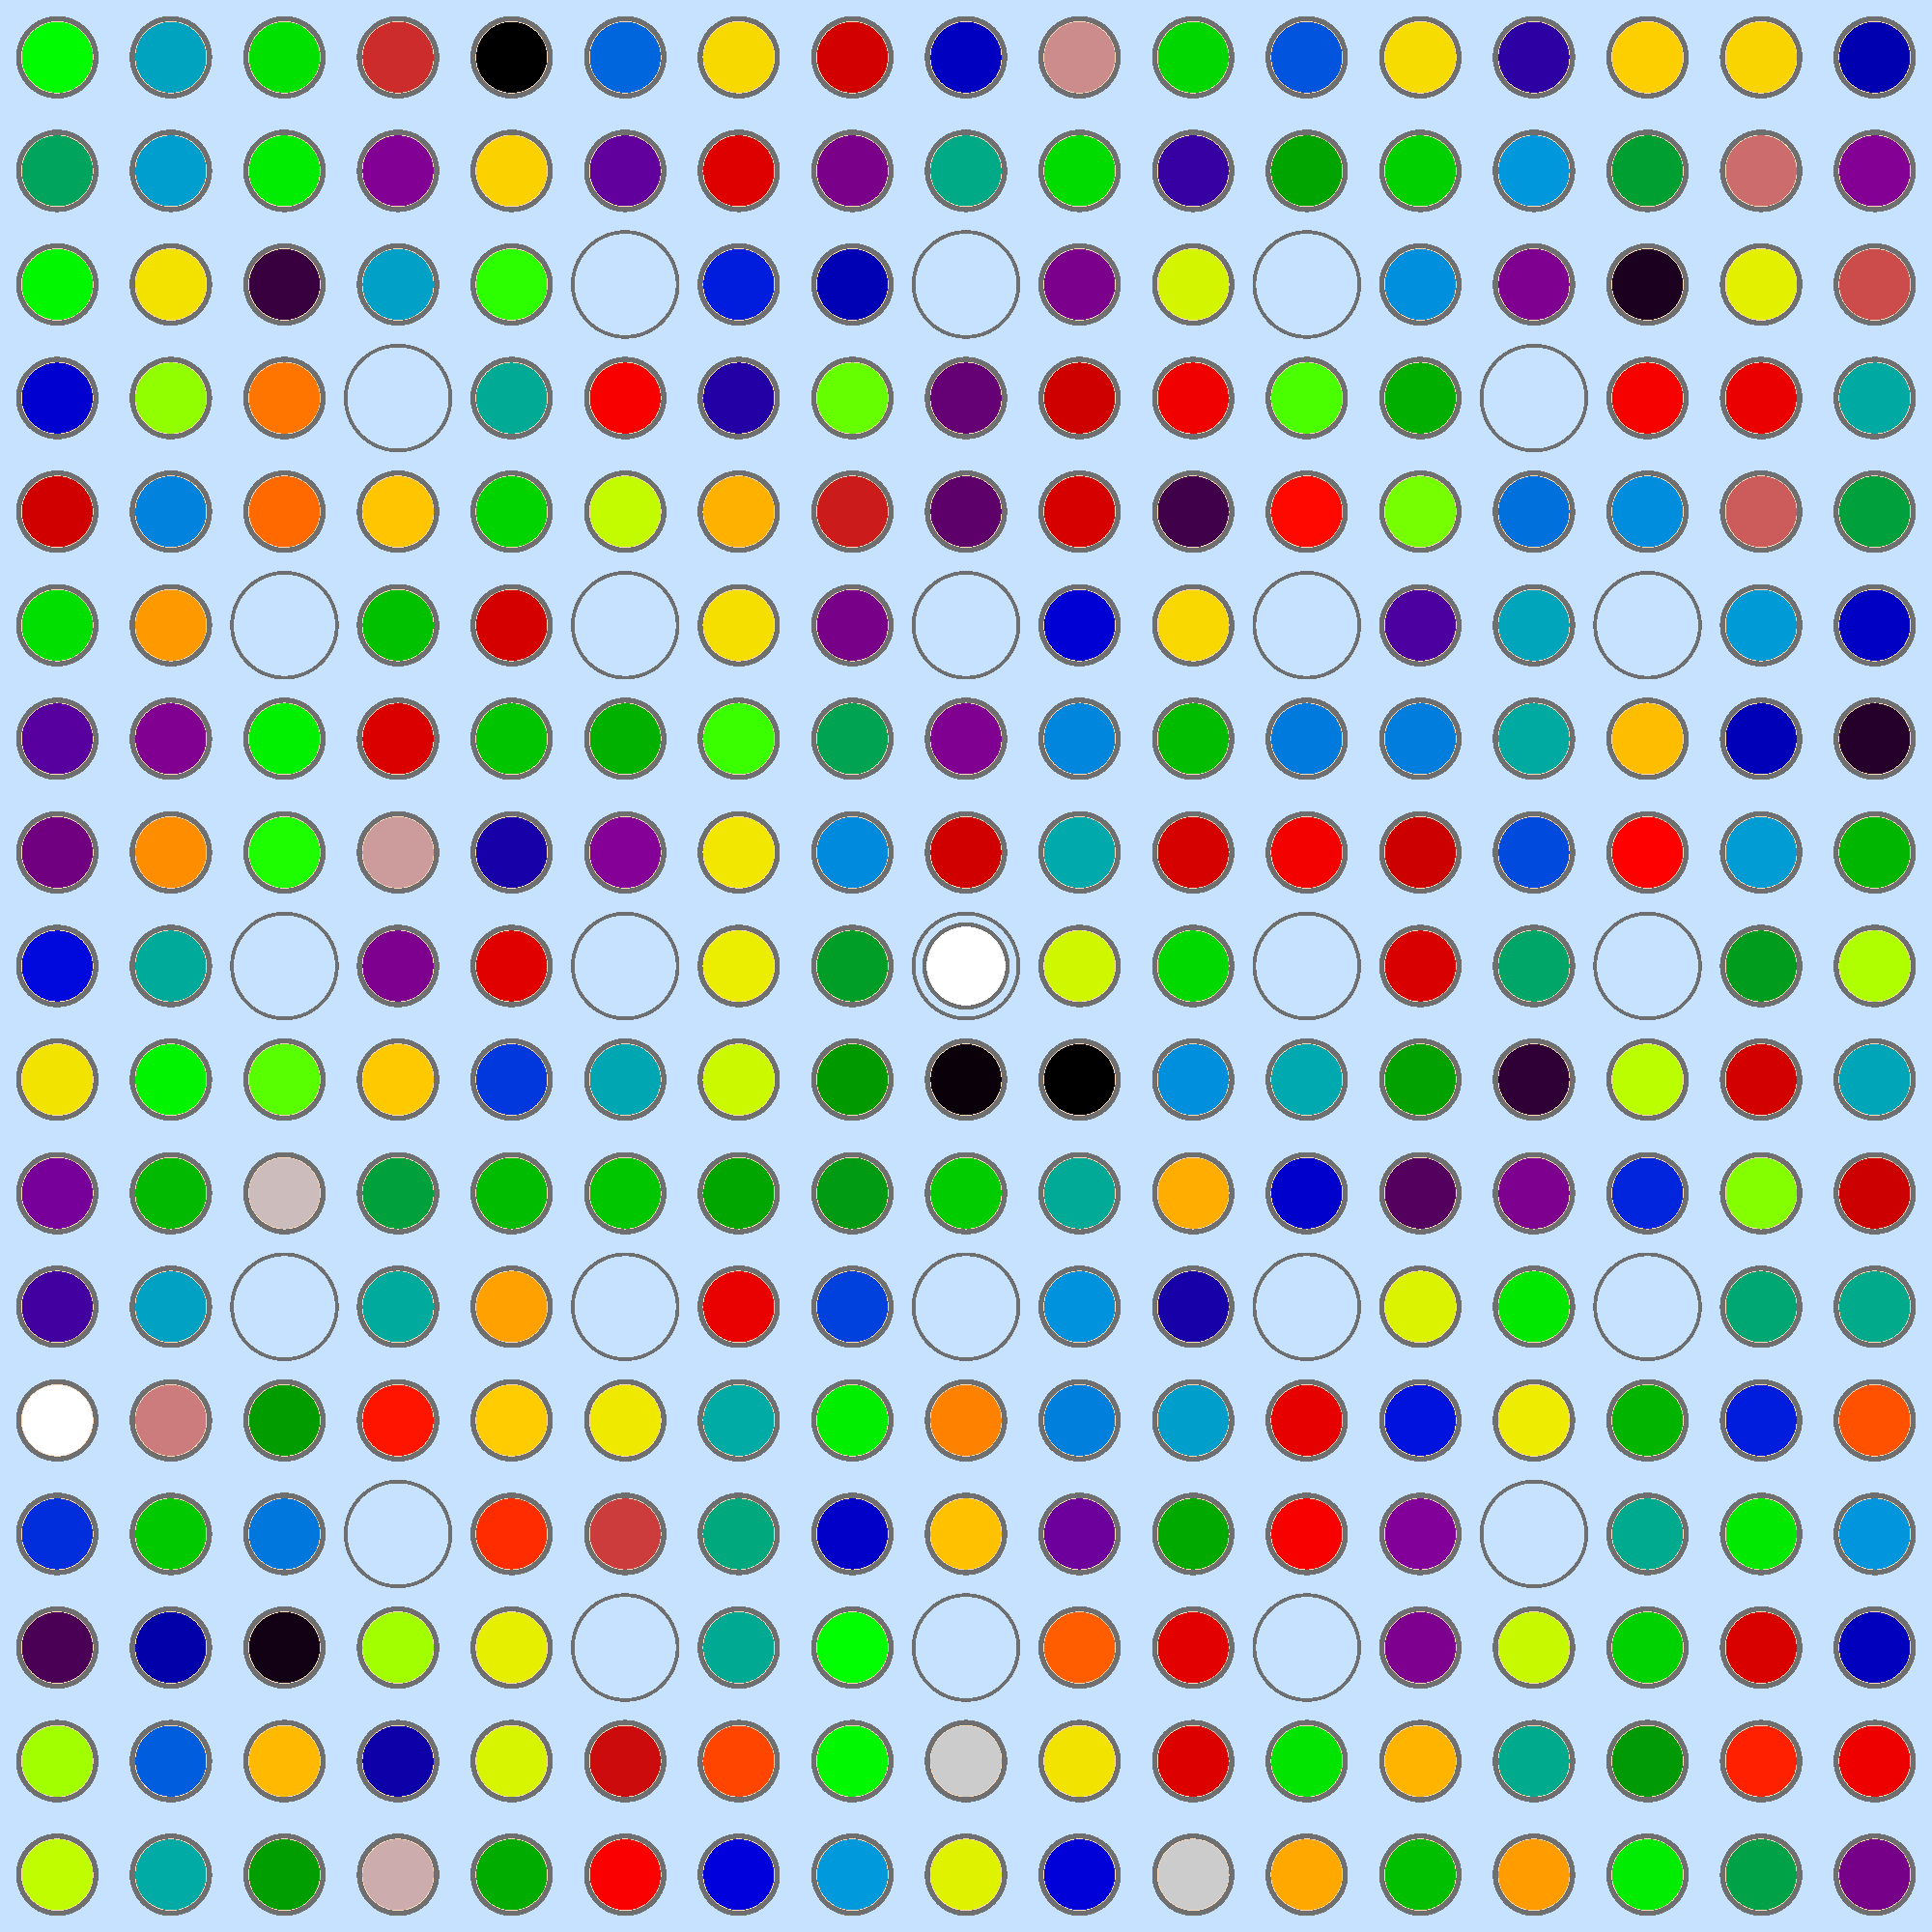
\includegraphics[width=0.8\linewidth]{figures/assembly/degenerate-materials}
  \caption{}
  \label{fig:degenerate-assm}
\end{subfigure}
\begin{subfigure}{0.45\textwidth}
  \centering
  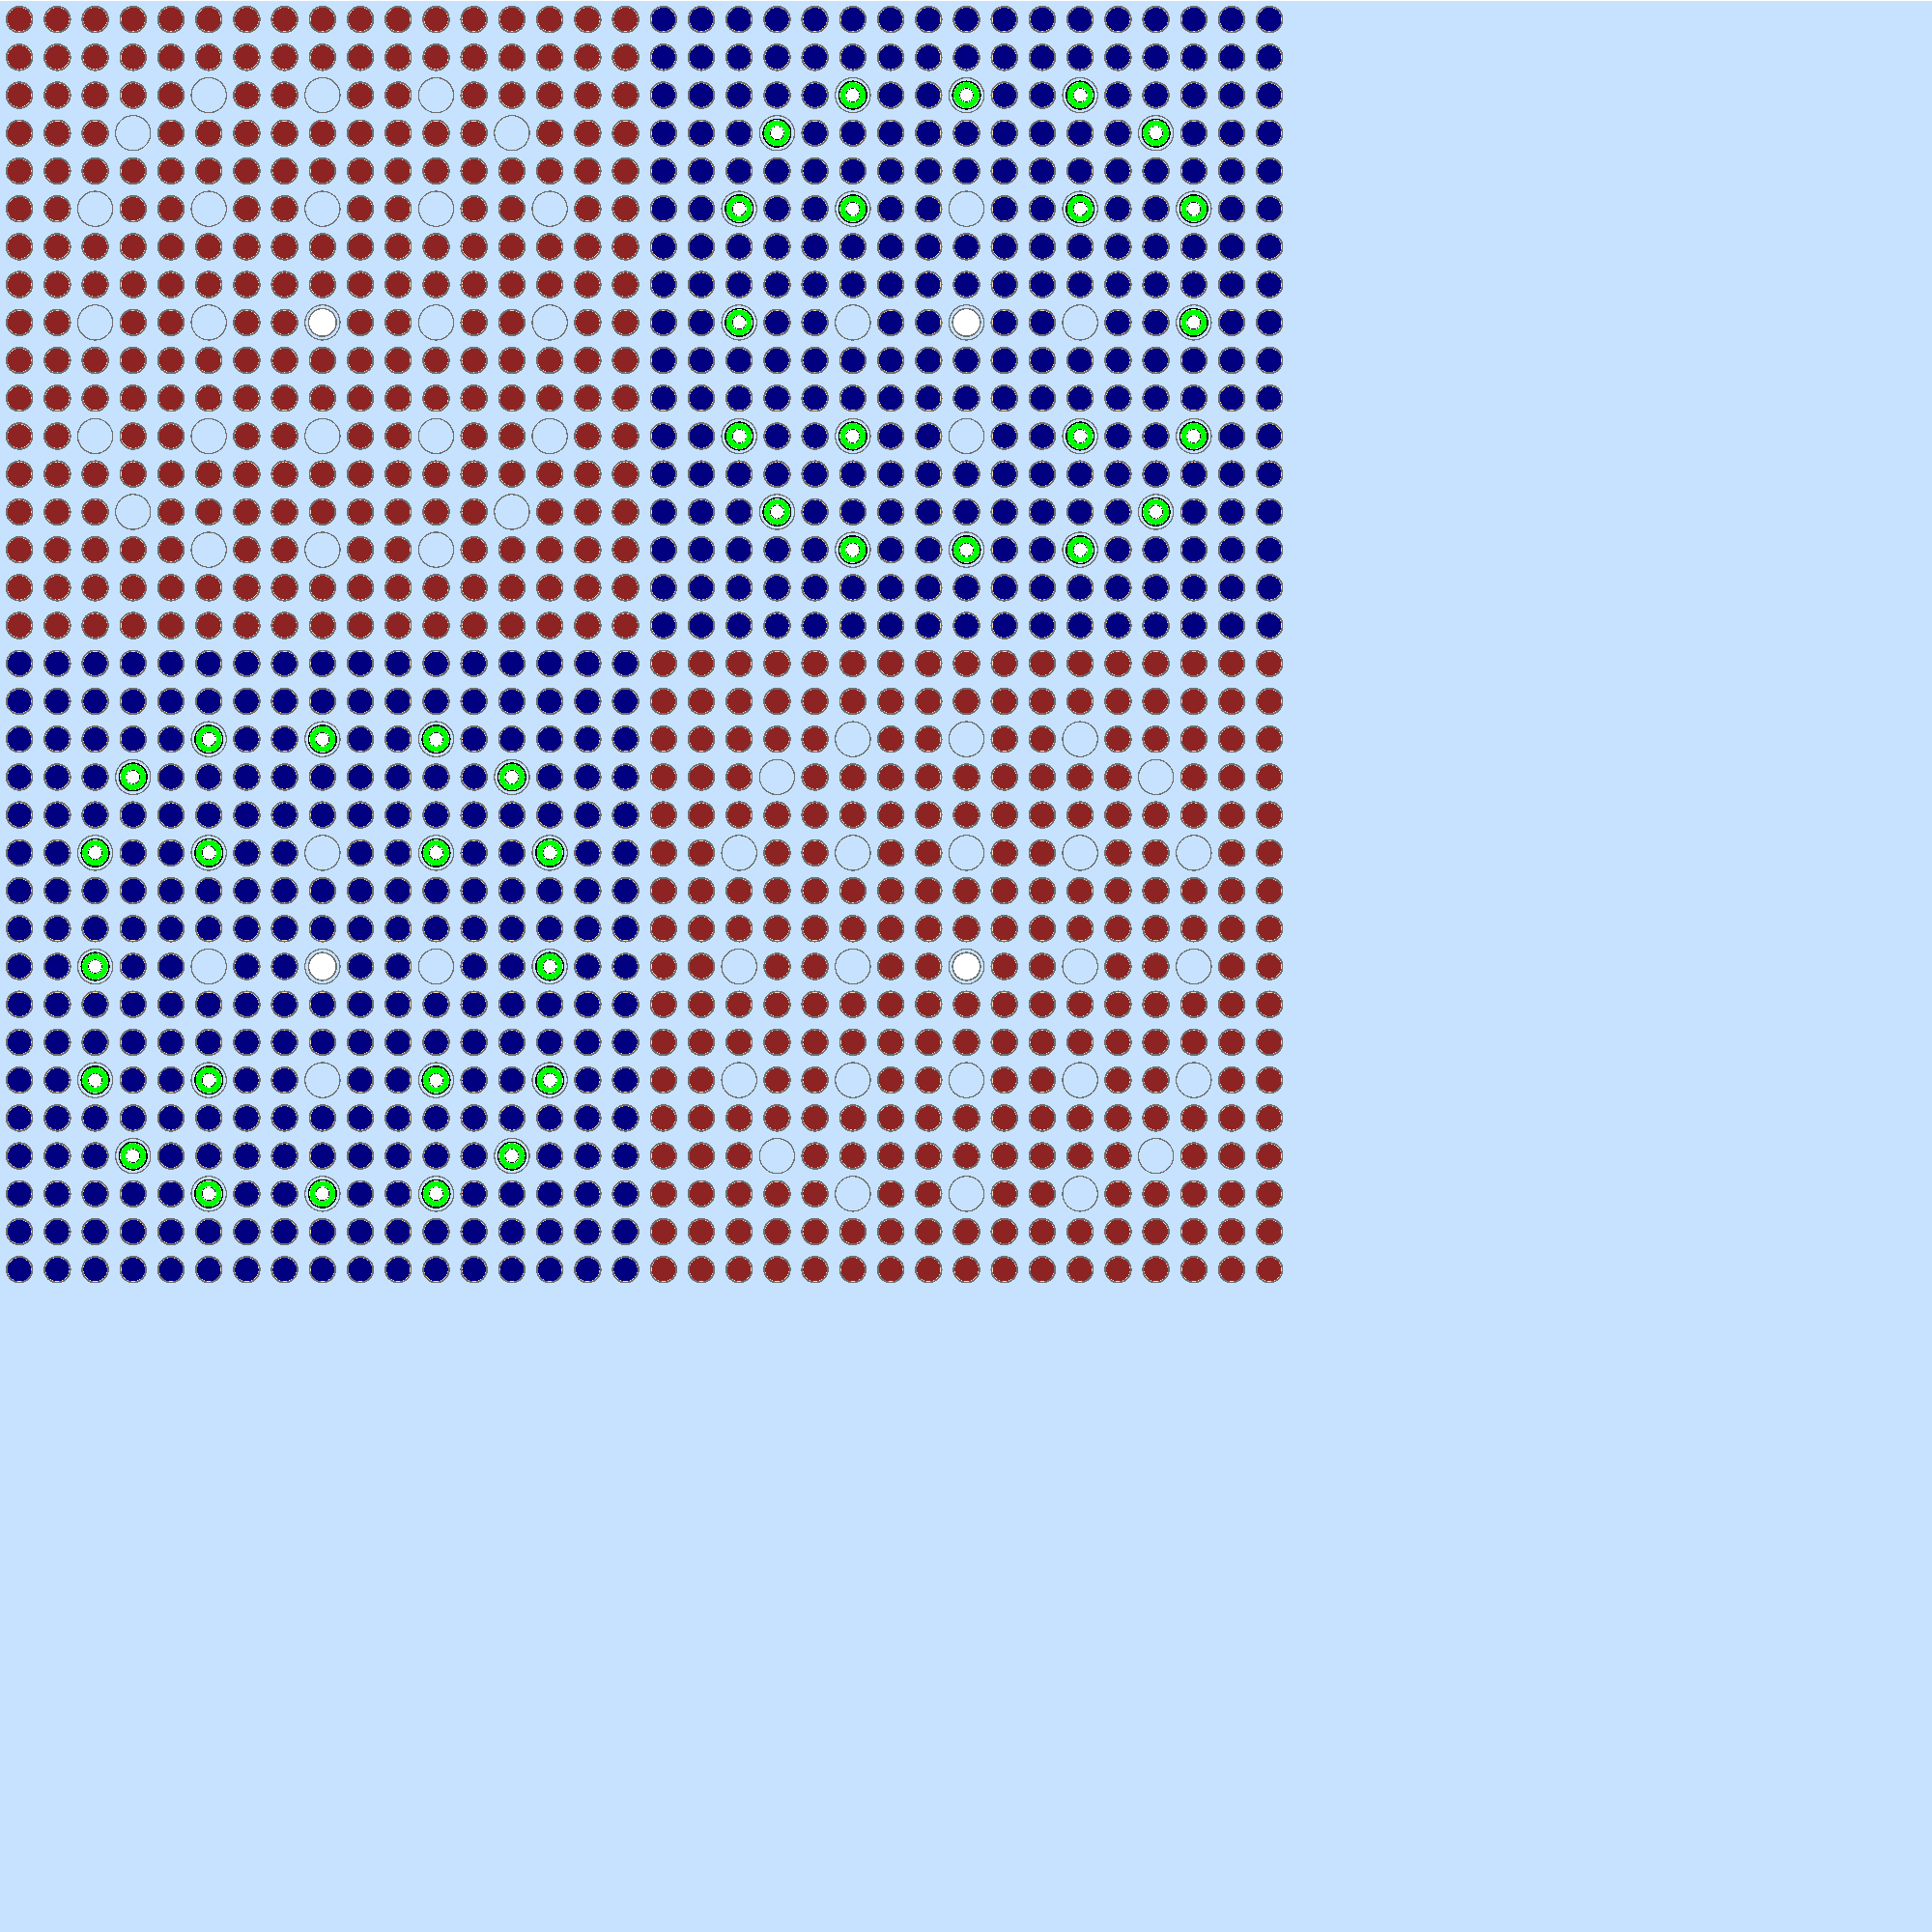
\includegraphics[width=0.8\linewidth]{figures/reflector/geometry}
  \caption{}
  \label{fig:null-reflector}
\end{subfigure}
\begin{subfigure}{0.45\textwidth}
  \centering
  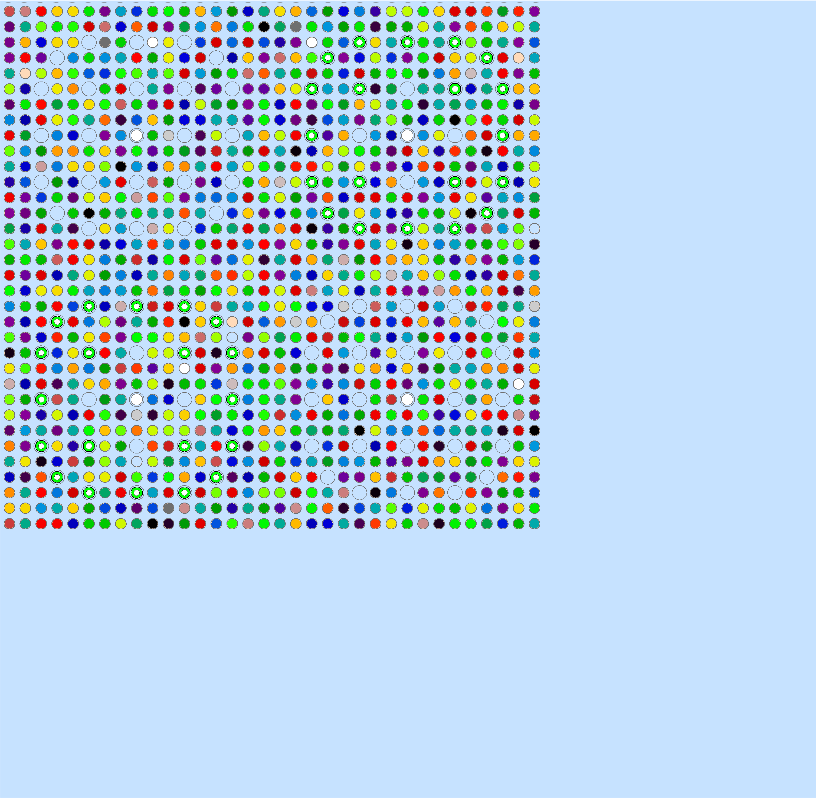
\includegraphics[width=0.8\linewidth]{figures/reflector/degenerate-materials}
  \caption{}
  \label{fig:degenerate-reflector}
\end{subfigure}
\caption{OpenMOC materials for the (a)-(b) assembly and (c)-(d) 2$\times$2 colorset models with null and degenerate homogenization, respectively.}
\label{fig:homogenization-schemes}
\end{figure*}

The \texttt{openmc.mgxs} module was used to compute 70-group MGXS with OpenMC for both the assembly and colorset benchmarks. The tallied MGXS data was condensed to coarse 2-group and 8-group structures with downstream data processing as necessary. The OpenMC simulations were performed with 1000 batches with 10$^{6}$ particle histories per batch for each benchmark. Stationarity of the fission source was obtained with 100 inactive batches for each benchmark. OpenMC's ``iso-in-lab'' feature was employed to enable consistent comparisons between OpenMC's reference results and OpenMOC's calculations with an isotropic in lab scattering source.

%%%%%%%%%%%%%%%%%%%%%%%%%%%%%%%%%%%%%%%%%%%%%%%%%%%%%%%%%%%%%%%%%%%%%%%%%%%%%%%
\subsubsection{Null Homogenization}
\label{subsubsec:homogenize-null}

The \textit{null} spatial homogenization scheme uses a single Monte Carlo calculation of the complete heterogeneous geometry to generate MGXS for each material. In this way, the null scheme fully abandons the multi-level approach used by most traditional approaches to generate MGXS. The spatially self-shielded flux is used to collapse the cross sections in each material with a unique isotopic composition. The null scheme does not account for spatial self-shielding effects experienced by different fuel pins filled by the same type of fuel, and instead averages these effects across the entire geometry. A single MGXS is employed in each instance of a material zone, such as a fuel pin replicated many times throughout a benchmark geometry.

%%%%%%%%%%%%%%%%%%%%%%%%%%%%%%%%%%%%%%%%%%%%%%%%%%%%%%%%%%%%%%%%%%%%%%%%%%%%%%%
\subsubsection{Degenerate Homogenization}
\label{subsubsec:homogenize-degenerate}

Unlike the null spatial homogenization scheme, the \textit{degenerate} scheme accounts for the different spatial self-shielding effects experienced by each instance of each fuel pin throughout a heterogeneous geometry. Like the null scheme, a single MC calculation of the complete heterogeneous geometry is used to generate MGXS for all materials. Unlike the null scheme, the MGXS are tallied separately for each instance of fissile material zones. For example, if a heterogeneous benchmark includes $N$ fuel pins, then $N$ collections of MGXS are separately tabulated for each fuel pin instance. The degenerate scheme tallies different MGXS even if the isotopic compositions in the fuel pin instances are identical (\textit{e.g.}, fresh fuel at the beginning of life) since each instance may experience different spatial self-shielding effects and hence have different MGXS.

The degenerate scheme generates MGXS for each fuel pin instance using OpenMC's distributed cell tallies~\citep{lax2014distribcell}. The OpenCG region differentiation algorithm~\citep{boyd2015opencg} is used to build a new OpenMOC geometry with unique cells and materials for each fuel pin. The MGXS are appropriately selected from OpenMC's distributed cell tallies to populate the MGXS in the OpenMOC materials. Multi-group transport calculations with MGXS generated using null and degenerate schemes may be compared to quantify the impact of modeling spatial self-shielding effects in MGXS for fissile zones in heterogeneous geometries.
%%%%%%%%%%%%%%%%%%%%%%%%%%%%%%%%%%%%%%%%%%%%%%%%%%%%%%%%%%%%%%%%%%%%%%%%%%%%%%%
\section{Conclusions}
\label{sec:conclusions}
%%%%%%%%%%%%%%%%%%%%%%%%%%%%%%%%%%%%%%%%%%%%%%%%%%%%%%%%%%%%%%%%%%%%%%%%%%%%%%%

Continuous energy Monte Carlo neutron transport methods have been increasingly applied for multi-group cross section generation. This paper introduced a single-step framework for MC-based MGXS generation for fine-mesh transport codes. The null and degenerate pin-wise spatial homogenization schemes were used to quantify the approximation error due to inter-pin spatial self-shielding effects in PWRs. The Local Neighbor Symmetry (LNS) pin-wise spatial homogenization was introduced to capture many of these self-shielding effects by homogenizing MGXS across groupings of fuel pins with similar neighboring spatial heterogeneities.

%The LNS scheme models spatial self-shielding with fewer materials than degenerate homogenization in order to accelerate the MC tally convergence rate by homogenizing MGXS across many fuel pins.

Two heterogeneous PWR benchmarks -- a fuel assembly and a 2$\times$2 assembly colorset with a water reflector -- were modeled in OpenMOC with MGXS generated by OpenMC. The single-step approach to MGXS generation was employed in which a single Monte Carlo eigenvalue calculation of the entire heterogeneous geometry was employed to collapse cross sections. Null spatial homogenization tallied MGXS for each fuel pin composition, while degenerate homogenization tallied MGXS for each unique fuel pin instance. LNS spatial homogenization applied a geometric template to group fuel pins with similar neighboring spatial heterogeneities. The eigenvalues, fission rates and U-238 capture rates predicted from multi-group calculations with OpenMOC were compared to a reference calculation with OpenMC for each of the three spatial homogenization schemes.

% The pin-wise U-238 capture rates, and to a lesser extent, the pin-wise fission rates, were better predicted when these effects were embedded into MGXS. 

The simulation results presented in this paper demonstrate that global reactivity is preserved when the same MC flux is used to collapse MGXS within a single-step MGXS generation scheme. The OpenMOC eigenvalues for each of the three pin-wise homogenization schemes are consistent to within 10 pcm. Hence, the choice of spatial homogenization technique is inconsequential to eigenvalue predictions. In contrast, the spatial homogenization scheme significantly impacts the accuracy of pin-wise reaction rate predictions. Non-negligible systematic approximation errors in the reaction rates arise when using MGXS which do not account for spatial self-shielding from neighboring fuel pins, control rod guide tubes and reflectors. Degenerate homogenization greatly reduced reaction rate errors with respect to null homogenization since it incorporated perturbations to the flux due to spatial heterogeneities. In particular, the maximum and mean U-238 capture rate errors were reduced by 2 -- 5$\times$ with degenerate homogenization. This demonstrated that the U-238 capture rate errors in deterministic multi-group transport calculations of PWRs are dominated by approximations to spatial self-shielding. In contrast, the fission rates were less sensitive to spatial self-shielding effects, and were only marginally reduced with degenerate homogenization.

LNS spatial homogenization performed as well as degenerate homogenization for a single assembly. However, the scheme failed to distinguish between pins at inter-assembly and assembly-reflector interfaces in the colorset, which resulted in a systematically large U-238 capture rate error for these fuel pins. The difficulty of generalizing the LNS algorithm for arbitrary geometries motivates the need for an unsupervised approach to accurately model spatial self-shielding effects. Such an approach should minimize the number of materials required to account for spatial self-shielding effects, and thus minimize the number of MC particle histories required to sufficiently converge MGXS statistical uncertainties.

%Although degenerate spatial homogenization was shown to be an effective approach to account for inter-pin spatial self-shielding, it is impractical for routine reactor analysis due to computational resource limitations. As a result of the fine-grained spatial tally mesh employed by degenerate homogenization, far more particle histories are needed to converge the MGXS tallies to obtain the same statistical uncertainties as with the simpler null scheme. Nevertheless, this analysis motivates the potential for a new spatial homogenization scheme as accurate as the degenerate scheme but requiring far fewer particle histories to converge MGXS.

%In general, the reaction rate errors for null homogenization are similar for groups of pins with similar neighboring heterogeneities. Hence, the errors may be equivalently reduced if an appropriate set of spatially self-shielded MGXS are defined for groups of pins with similar flux profiles. Future work should develop methods which best identify groups of pins to homogenize to achieve the accuracy of the degenerate scheme while simultaneously approaching the MC convergence rate of the null scheme. This is a topic of ongoing investigation and will be presented in future publications.

%%%%%%%%%%%%%%%%%%%%%%%%%%%%%%%%%%%%%%%%%%%%%%%%%%%%%%%%%%%%%%%%%%%%%%%%%%%%%%%
\section*{Acknowledgments}
%%%%%%%%%%%%%%%%%%%%%%%%%%%%%%%%%%%%%%%%%%%%%%%%%%%%%%%%%%%%%%%%%%%%%%%%%%%%%%%


This work was supported by the Idaho National Laboratory and the National Science Foundation Graduate Research Fellowship Grant No. 1122374. This research made use of the resources of the High Performance Computing Center at Idaho National Laboratory, which is supported by the Office of Nuclear Energy of the U.S. Department of Energy and the Nuclear Science User Facilities under Contract No. DE-AC07-05ID14517.

\section*{References}
\bibliography{references}
\bibliographystyle{annals}

\end{document}
